\documentclass[12pt,a4paper]{article}

%%%%%%%%%%%%%%%%%%%%%PAQUETES%%%%%%%%%%%%%%%%%%%%%%%%%%%%%%%%%%%
\usepackage[utf8]{inputenc} %Codificación
\usepackage[spanish]{babel} %Idioma español
\usepackage[right=2cm,left=2cm,top=2cm,bottom=2cm]{geometry} %Control de márgenes
\usepackage{hyperref}%Introducir enlaces
\usepackage{fancyhdr}%Encabezados y pie de página
\usepackage{listing}%Inserción de código
\usepackage{color}
\usepackage[export]{adjustbox}
\usepackage{graphicx}
\usepackage{float}
\usepackage{changepage}
%%%%%%%%%%%%%%%%%%%%%%COMANDOS%%%%%%%%%%%%%%%%%%%%%%%%%%%%%%%%%%%

\pagestyle{fancy}%Estilo de pie página y encabezados
\renewcommand{\footrulewidth}{0.4pt}
\setlength{\headheight}{15pt}
\fancyhead[L]{Entornos de Desarrollo}
\fancyhead[R]{Juan Miguel Rivas Velasco}
\fancyfoot[L]{IES Francisco de los Ríos}
\fancyfoot[R]{1º CSFP DAM}

%%%%%%%%%%%%%%%%%%%%Definición de colores%%%%%%%%%%%%%%%%%%%%%%%%
\definecolor{prussianblue}{rgb}{0.0, 0.19, 0.33}


%%%%%%%%%%%%%%%%%%%Documento%%%%%%%%%%%%%%%%%%%%%%%%%%%%%%%%%%%%%

\begin{document}

\begin{titlepage}
    \vspace{0.5 cm}
    \begin{center}
        \frame{
\includegraphics[width=\textwidth]{logo2.png}}
    \end{center}
    \vspace{1 cm}
    \rule{\textwidth}{1mm}
    \begin{center}
        \large \bfseries \textcolor{prussianblue}{MEDIEVAL GAME}
    \end{center}
    \rule{\textwidth}{1mm}
    \vspace{0.8cm}

    \begin{center}
        \frame{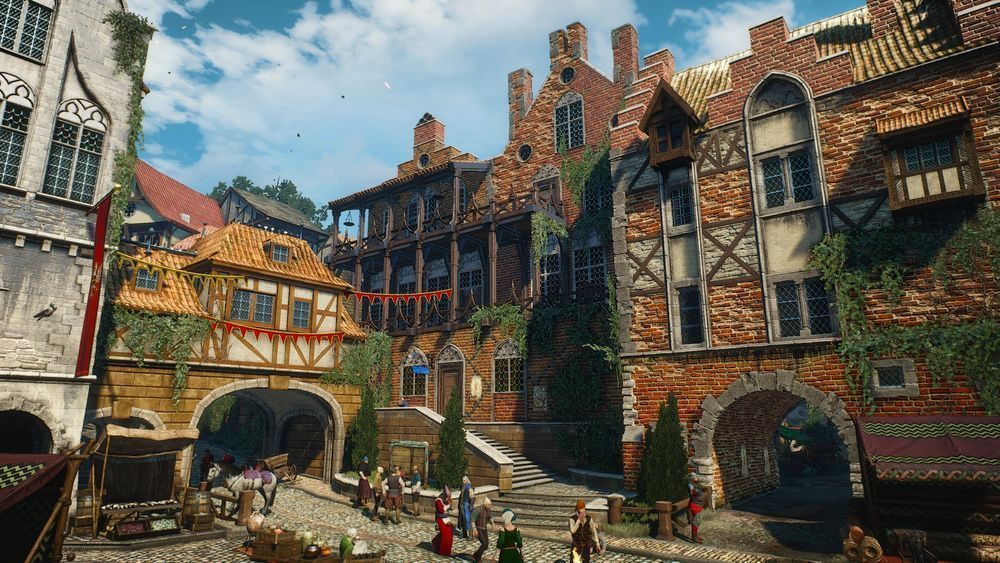
\includegraphics[scale=0.45]{novigrado.jpg}}
    \end{center}
    \vspace{1cm}
    \rule{\textwidth}{1mm}
    \vspace{1cm}

    \hspace{1.2cm}
    
    \hspace{1cm}
    \begin{minipage}[b]{0.7\textwidth}
        \textbf{\normalsize\textcolor{prussianblue}{Asignatura:}} \normalsize{Entornos de Desarrollo}

        \textbf {\normalsize\textcolor{prussianblue}{Curso:}} \normalsize{1º CSFP Desarrollo de aplicaciones multiplataforma}

        \textbf{\normalsize \textcolor{prussianblue}{Estudiantes:}} \normalsize{Juan Miguel, Alejandro, Antonio, Pedro, Raul }

        \textbf{\normalsize \textcolor{prussianblue}{Profesor:}} \normalsize{Miguel Morales Carmona}
    \end{minipage}


    \vspace{1 cm}

    \begin{center}
        \textbf{\small \textcolor{prussianblue}{Fecha:}} \small{\today}

        \vfill
    \end{center}
\end{titlepage}

\begin{abstract}
    Diseñar en editor Dia las clases que cada uno tenga asignadas. Cada uno debe subir al GitHub un único archivo .dia con todas sus clases en él,
    con el formato nombreDiagramas.dia ; Ejemplo: JuanMiguelDiagramas.dia 
    \newline
    Así mismo las subidas se realizaran a través de git mediante claves ssh y no de forma manual. Para ello debeis crear una clave ssh en cada ordenador que useis y añadirlo 
    a vuestra cuenta de github.
    \newline
    \textbf{Enlace a Github: }\href{https://github.com/juanmirivas8/MedievalGame}{https://github.com/juanmirivas8/MedievalGame}
    \newline 
    \textbf{Instrucciones: }
    \begin{enumerate}
        \item git init
        \item git remote add \textit{origin} git@github.com:juanmirivas8/MedievalGame.git
    \end{enumerate}
    

\end{abstract}

\tableofcontents
\newpage
\raggedright 

\section{Antonio}
    \subsection{Clase Ciudad}
    \paragraph{}
    Ésta clase representa a una ciudad y contiene todos los atributos y métodos necesarios para modelarla
        \subsubsection{Atributos}
        \begin{itemize}
            \item \textbf{private Double ingresos}
            \item \textbf{private Double oro}
            \item \textbf{private ArrayList$<$Deuda$>$ listaDeudas}
            \item \textbf{private Double inflacion}
            \item \textbf{private Integer estabilidad}
            \item \textbf{private Double agitacion}
            \item \textbf{private Integer soldadesca} 
            \item \textbf{private PuebloHumano humanos}
            \item \textbf{private Poblacion humanos} 
            \item \textbf{private Poblacion nohumanos}
            \item \textbf{private Double mantenimientoEjercito}
            \item \textbf{private Double mantenimientoAdministracion}
            \item \textbf{private ArrayList$<$Privilegio$>$ listaPoliticas}
            \item \textbf{private ArrayList$<$Edificio$>$ listaEdificios}
            \item \textbf{private ArrayList$<$Evento$>$ eventosActivos}
            \item \textbf{private Double modificadorImpuestos}
            \item \textbf{private Double modificadorSoldadesca}
            \item \textbf{private Double corrupcion}
            \item \textbf{private Double propiedadPublica}
        \end{itemize}
        \subsubsection{Metodos}
        \begin{itemize}
            \item \textbf{public getGastos()}
            \item \textbf{public getRecaudacion()}
            \item \textbf{public getIngresos()}
            \item \textbf{Resto de getters y setters publicos}
        \end{itemize}

\section{Alejandro}
    \subsection{Clase Poblacion}
    \paragraph{}
    Clase que representa un estamento y contiene todos los atributos y métodos para manejarlos.
            \subsubsection{Atributos}
            \begin{itemize}
                \item \textbf{protected String nombre}
                \item \textbf{protected Integer Cantidad}
                \item \textbf{protected Double influencia}
                \item \textbf{protected Double propiedadPrivada}
                \item \textbf{protected Double modificadorImpuestos}
                \item \textbf{protected Double modificadorSoldadesca}
                \item \textbf{protected Integer maximaSoldadesca}
                \item \textbf{protected Double crecimiento}
                \item \textbf{private ArrayList$<$Privilegio$>$ listaPrivilegios}
            \end{itemize}
            \subsubsection{Metodos}
            \begin{itemize}
                \item \textbf{Getters y setters publicos}
            \end{itemize}
\section{Raul}
    \paragraph{}
    Ésta clase simula un préstamo que se pide. Tiene un interés, el cual determina cuanto se paga al final y cada turno. 
    \subsection{Clase Deuda}
        \subsubsection{Atributos}
        \begin{itemize}
            \item \textbf{private Double importe}
            \item \textbf{private Double interes}
        \end{itemize}
        \subsubsection{Metodos}
        \begin{itemize}
            \item \textbf{public Double getImporte()}
            \item \textbf{public void setImporte()}
            \item \textbf{public Double getInteres()}
            \item \textbf{public Double setInteres()} 
        \end{itemize}
    \paragraph{}
    Clase abstracta la cual será implementada por diferentes tipos de edificios, los cuales tendrán distintos efectos y costes.
    \subsection{Clase Edificio (Abstracto)}
        \subsubsection{Atributos}
        \begin{itemize}
            \item \textbf{private Double precio}
            \item \textbf{private Double precioVenta} 
            \item \textbf{private String Descripcion}
        \end{itemize}
        \subsubsection{Metodos}
        \begin{itemize}
            \item \textbf{public String aplicarEfecto(Ciudad c)}
            \item \textbf{public String revertirEfecto(Ciudad c)}
            \item \textbf{Getters y setters de los otros atributos}
        \end{itemize}

        \subsection{Clase Controlador}
        \paragraph{}
        Controlador del programa que coordina la vista con el modelo, el cual es una clase de tipo partida.
        \subsubsection{Atributos}
        \begin{itemize}
            \item \textbf{private Vista v}
            \item \textbf{private Partida p}
        \end{itemize}
        \subsubsection{Metodos}
        \begin{itemize}
            \item \textbf{public void run()}
            \item \textbf{metodos privados}
        \end{itemize}
        
\section{Pedro}
    \paragraph{} 
    Clase Privilegio, el cual ofrece una serie de beneficios a aquella entidad que lo posea, ya sea el gobernante o alguna población.
    \subsection{Clase Privilegio (Abstracta)}
        \subsubsection{Atributos}
            \begin{itemize}
                \item \textbf{private String Descripcion}
            \end{itemize}
        \subsubsection{Metodos}
        \begin{itemize}
            \item \textbf{public String aplicarEfecto(Ciudad c)}
            \item \textbf{public String revertirEfecto(c)}
            \item \textbf{Resto de getters y setters} 
        \end{itemize}
    \subsection{Clase Evento (Abstracta)}
    \paragraph{}
    Clase abstracta que luego será implementado por diferentes eventos, tanto positivos como negativos. Los eventos pueden ser lanzados
    aleatoriamente o también si se cumplen una serie de condiciones.
        \subsubsection{Atributos}
        \begin{itemize}
            \item \textbf{private Integer turnosRestantes}
            \item \textbf{private String Descripcion}
        \end{itemize}
        \subsubsection{Metodos}
        \begin{itemize}
            \item \textbf{public String aplicarEvento(Ciudad c)}
            \item \textbf{public String revertirEvento(c)}
            \item \textbf{Getters y setters}
        \end{itemize}
        \subsection{Clase Vista}
        \paragraph{}
        La clase vista contendrá multitud de métodos de entrada y salida para la correcta interacción del programa con el usuario.
        \subsubsection{Metodos}
        \begin{itemize}
            \item \textbf{Metodos de lectura y escritura}
        \end{itemize}

\section{Juan Miguel}
    \subsection{Clase }
        \subsubsection{Atributos}
        \begin{itemize}
        \item \textbf{private Ciudad c} 
        \item \textbf{private ArrayList$<$Evento$>$ listaEventos}
        \end{itemize}
    \subsubsection{Metodos}
        \begin{itemize}
        \item \textbf{Multitud eventos funcionamiento: }pagarDeuda, lanzarEventoAleatorio, darPrivilegio, etc
        \end{itemize}
    


\end{document}